% this file is called up by thesis.tex
% content in this file will be fed into the main document
\chapter{Complementos}
% top level followed by section, subsection

\section{Lectura de listas}
\label{lectura.listas}
 
Las listas hechas para los préstamos nuevos \cite{prestamos_nuevos} y los préstamos acumulados \cite{prestamos_acumulados} de un idioma origen \textit{A} en un receptor \textit{B},  se encuentran ordenadas por cada año de la base de datos (1740-2009), y a la vez en cada año, las palabras listadas se ordenaron de forma descendente en frecuencia $f$ y ascendente en rango $k$; entonces en el año $t$, la palabra más frecuente tiene rango $k=1$, la segunda más frecuente  tiene rango $k=2$, y así sucesivamente para todas las palabras en ese año. 


Si para el año $t$  se encontraron $n$ cantidad de palabras, cuyas frecuencias cumplen que $f_{1} > f_{2} > f_{3} >  \dots > f_{n-1} > f_{n}$,  entonces el ordenamiento es el siguiente. 
\begin{table}[h!]
	\centering
	\begin{tabular}{ccc}
		\multicolumn{3}{c}{\textbf{Año $t$}}          \\
		Rango $k$     & Palabra    & Frecuencia $f$    \\
		1             & pal 1      & $f_{1}$            \\
		2             & pal 2      & $f_{2}$             \\
		3             & pal 3      & $f_{3}$              \\
		$\vdots$      & $\vdots$   & $\vdots$         \\
		$\vdots$      & $\vdots$   & $\vdots$         \\
		$n-1$         & pal $n-1$  & $f_{n-1}$             \\
		$n$           & pal $n$    & $f_{n}$          
	\end{tabular}
\end{table}
Para su mejor lectura y evitar confusiones con los números,  se omitieron las frecuencias en los listados. 








\section{Gráficas de palabras acumuladas entre dos idiomas}
\label{palabras.acumuladas.apendice}

\begin{figure}[h!]
	\centering
	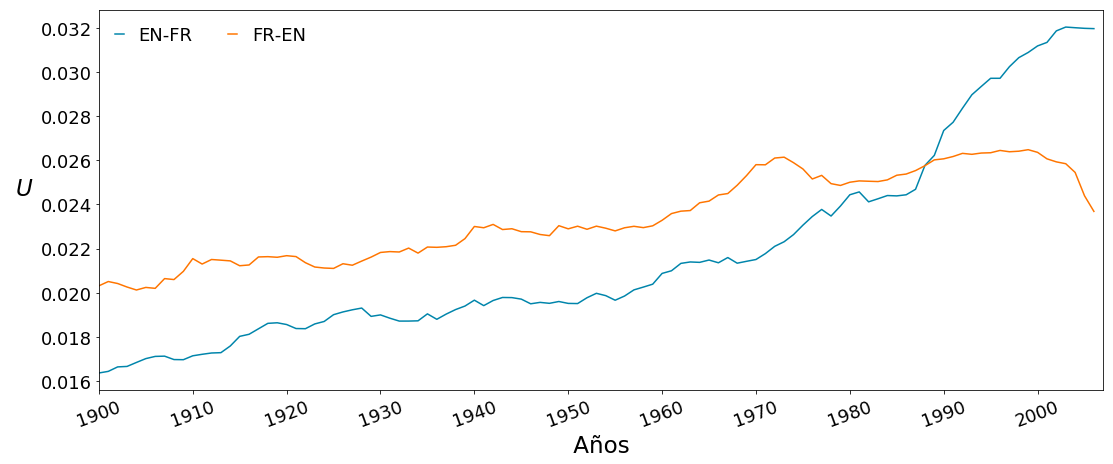
\includegraphics[scale=.38]{UOR_1EN.png}
	\label{fig.U_EF}
	\caption{Palabras acumuladas entre el inglés y el francés}
\end{figure}


\begin{figure}[h!]
	\centering
	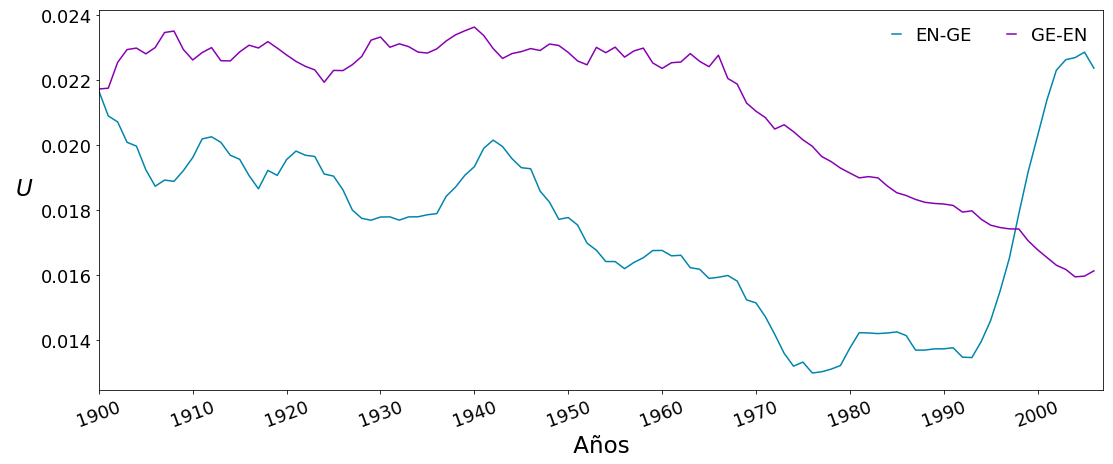
\includegraphics[scale=.38]{UOR_2EN.png}
	\label{fig.U_EG}
	\caption{Palabras acumuladas entre el inglés y el alemán}
\end{figure}


\begin{figure}[h!]
	\centering
	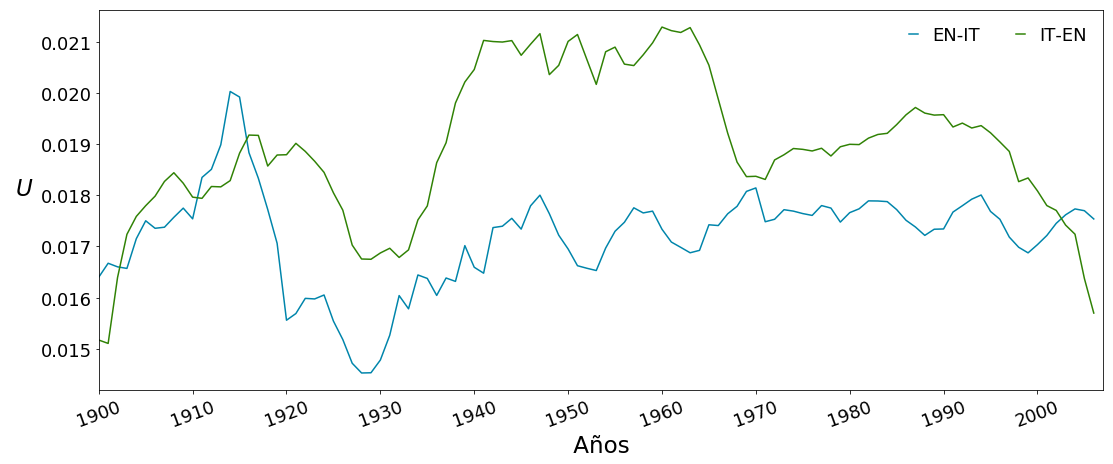
\includegraphics[scale=.38]{UOR_3EN.png}
	\label{fig.U_EI}
	\caption{Palabras acumuladas entre el inglés y el italiano}
\end{figure}

\begin{figure}[h!]
	\centering
	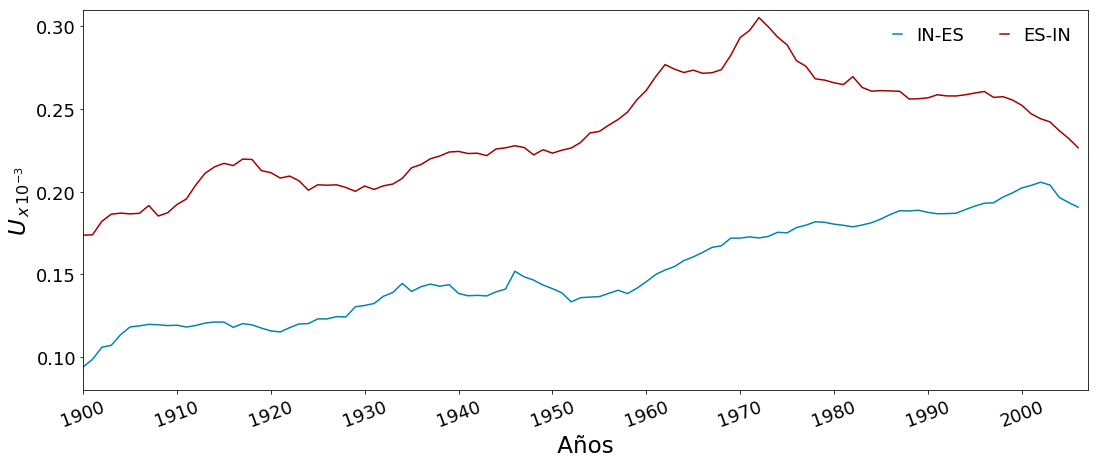
\includegraphics[scale=.38]{UOR_4EN.png}
	\label{fig.U_ES}
	\caption{Palabras acumuladas entre el inglés y el español}
\end{figure}

\begin{figure}[h!]
	\centering
	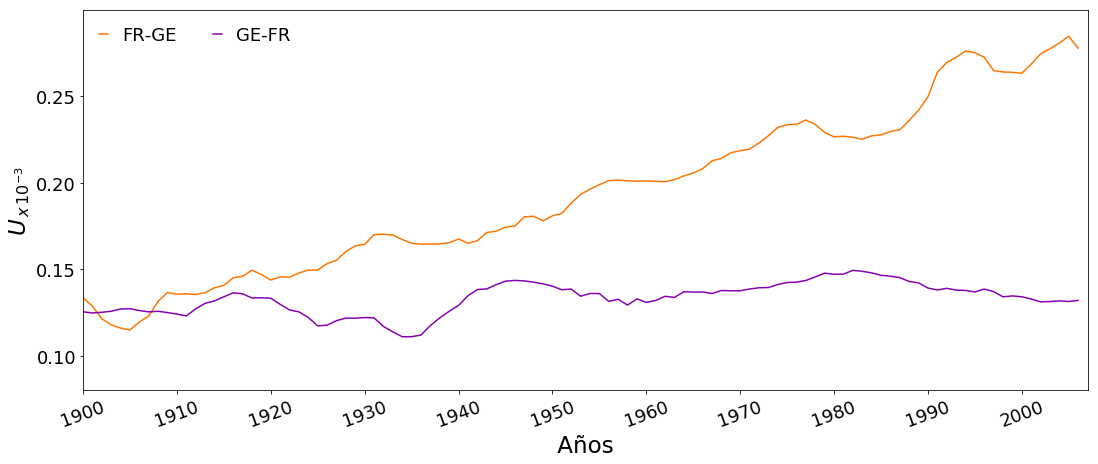
\includegraphics[scale=.38]{UOR_1FR.png}
	\label{fig.U_FG}
	\caption{Palabras acumuladas entre el francés y el alemán}
\end{figure}

\begin{figure}[h!]
	\centering
	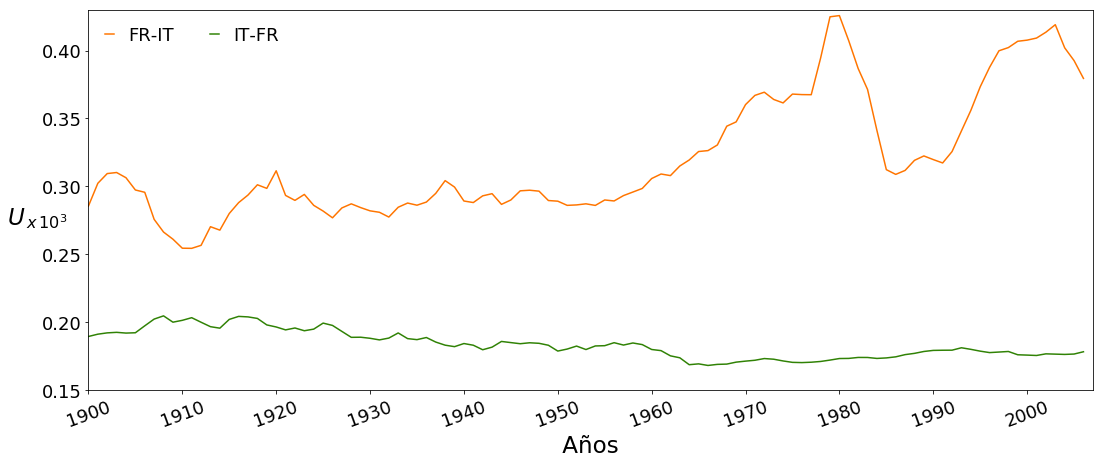
\includegraphics[scale=.38]{UOR_2FR.png}
	\label{fig.U_FI}
	\caption{Palabras acumuladas entre el francés y el italiano}
\end{figure}

\begin{figure}[h!]
	\centering
	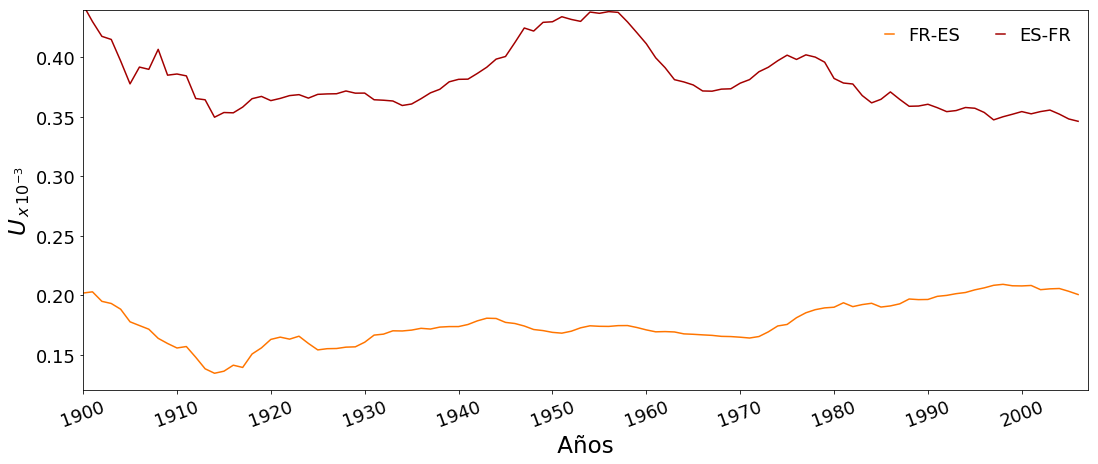
\includegraphics[scale=.38]{UOR_3FR.png}
	\label{fig.U_FS}
	\caption{Palabras acumuladas entre el francés y el español}
\end{figure}



\begin{figure}[h!]
	\centering
	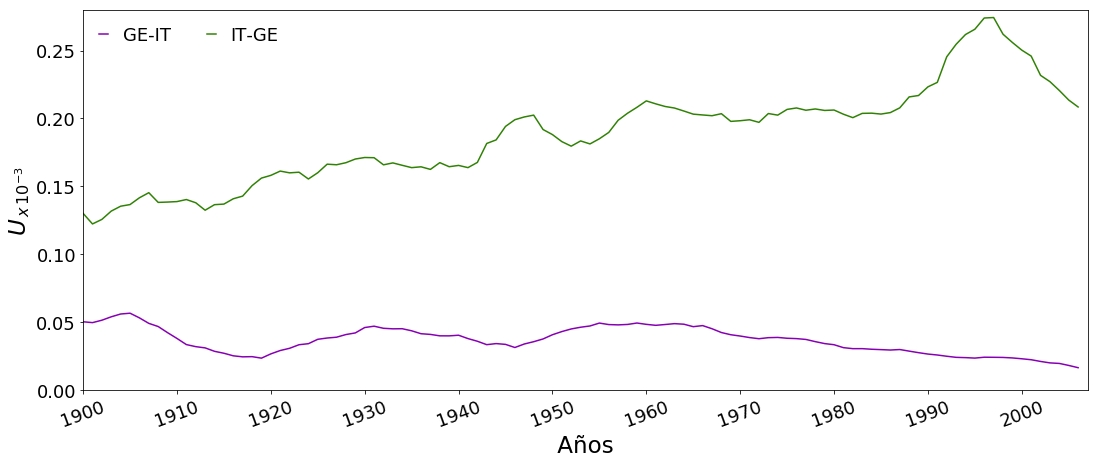
\includegraphics[scale=.38]{UOR_1GE.png}
	\label{fig.U_GI}
	\caption{Palabras acumuladas entre el alemán y el italiano}
\end{figure}


\begin{figure}[h!]
	\centering
	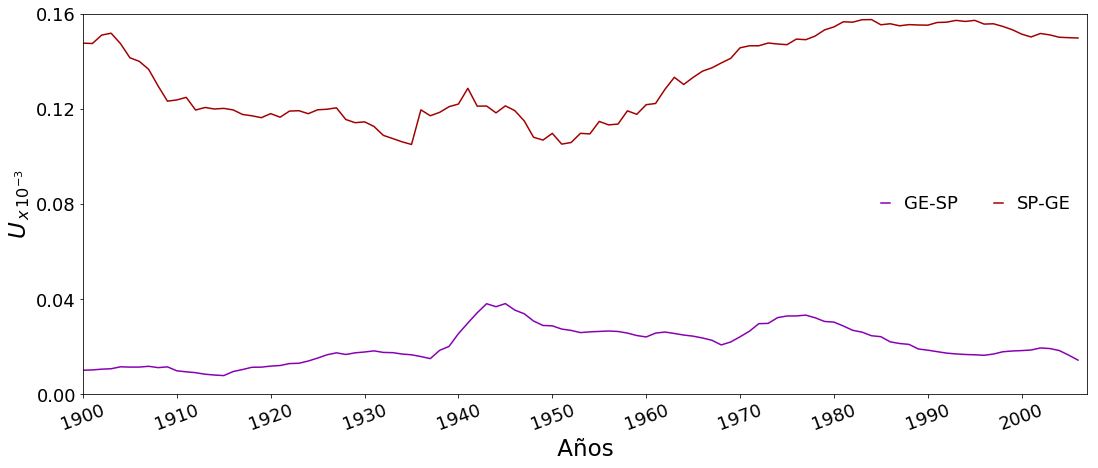
\includegraphics[scale=.38]{UOR_2GE.png}
	\label{fig.U_GS}
	\caption{Palabras acumuladas entre el alemán y el español}
\end{figure}


\begin{figure}[h!]
	\centering
	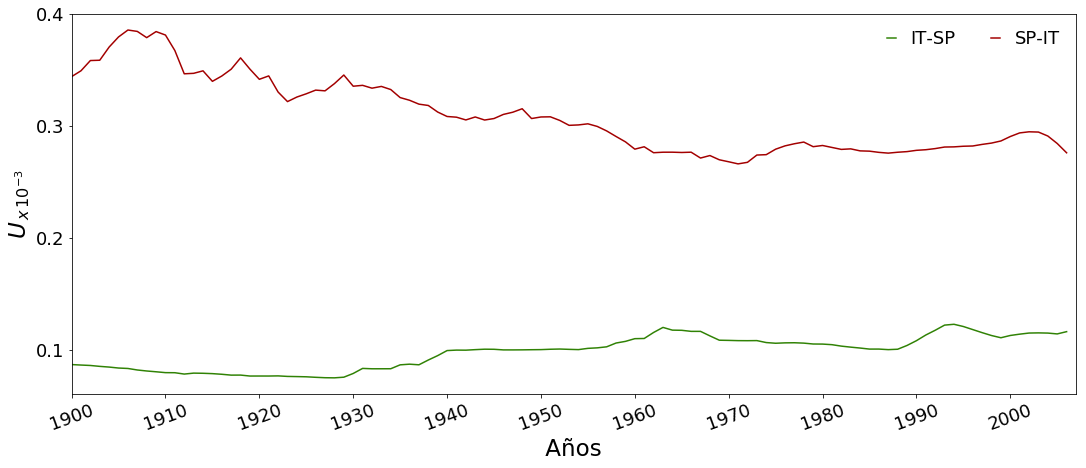
\includegraphics[scale=.38]{UOR_1IT.png}
	\label{fig.U_IS}
	\caption{Palabras acumuladas entre el italiano y el español}
\end{figure}

%\section{Eliminación de palabras}
%\label{eliminacion.completa.apendice}


